\documentclass[tikz,11pt]{standalone}
\usepackage{textcomp}

\usepackage{tikz}
\usetikzlibrary{shapes.geometric, arrows}
\usepackage{xcolor}

% Custom colors
\definecolor{backcolour}{rgb}{0.95,0.95,0.92}
\definecolor{backcolour}{RGB}{229, 229, 229}
% Polar Night Palette
\definecolor{nightDarkest}{RGB}{46, 52, 64}
\definecolor{nightDark}{RGB}{59, 66, 82}
\definecolor{nightMid}{RGB}{67, 76, 94}
\definecolor{nightLight}{RGB}{76, 86, 106}
% Snow Storm Palette
\definecolor{snowDark}{RGB}{216, 222, 233}
\definecolor{snowMid}{RGB}{229, 233, 240}
\definecolor{snowLight}{RGB}{236, 239, 244}
% Frost Palette
\definecolor{frostTurqoise}{RGB}{143, 188, 187}
\definecolor{frostLightBlue}{RGB}{136, 192, 208}
\definecolor{frostMidBlue}{RGB}{129, 161, 193}
\definecolor{frostDarkBlue}{RGB}{94, 129, 172}
% Aurora Palette
\definecolor{auroraLila}{RGB}{180, 142, 173}
\definecolor{auroraRed}{RGB}{191, 97, 106}
\definecolor{auroraOrange}{RGB}{208, 135, 112}
\definecolor{auroraYellow}{RGB}{235, 203, 139}
\definecolor{auroraGreen}{RGB}{163, 190, 140}

% Baskervald X for roman, with oldstyle figure
\usepackage[osf]{Baskervaldx}
% load amssymb before newtxmath to avoid problem with \Bbbk
\usepackage{amssymb}
% Nice math calligraphic font 
\usepackage[cal=boondoxo]{mathalpha}
% Math font to match
\usepackage[bigdelims,baskervaldx]{newtxmath}

% \usetikzlibrary{backgrounds}

\begin{document}


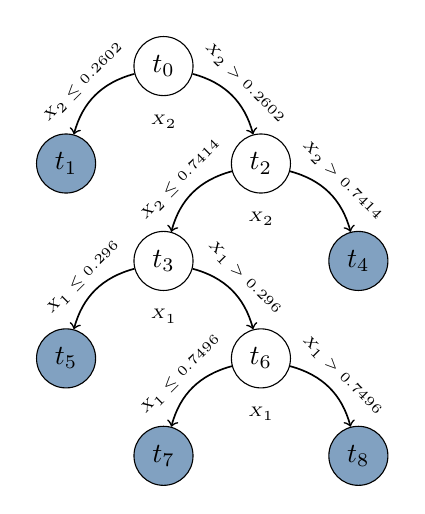
\begin{tikzpicture}
    [
		% show background rectangle,
		node distance=1.75cm,
		place/.style={
			draw, circle, align=center, minimum size=0.75cm, fill=white
		},
		nodet/.style={
			draw, circle, align=center, minimum size=0.75cm, fill=frostMidBlue
		}
	]

% Nodes
\node (root) [place, align=center] {$t_0$};
\node [below of=root, node distance = 20pt] {\tiny $X_2$};
\node (t1) [nodet, below left of=root] {$t_1$};
\node (t2) [place, below right of=root] {$t_2$};
\node [below of=t2, node distance = 20pt] {\tiny $X_2$};
\node (t3) [place, below left of=t2] {$t_3$};
\node (t4) [nodet, below right of=t2] {$t_4$};
\node (t5) [nodet, below left of=t3] {$t_5$};
\node [below of=t3, node distance = 20pt] {\tiny $X_1$};
\node (t6) [place, below right of=t3] {$t_6$};
\node [below of=t6, node distance = 20pt] {\tiny $X_1$};
\node (t7) [nodet, below left of=t6] {$t_7$};
\node (t8) [nodet, below right of=t6] {$t_8$};

% Transitions
\draw [->, semithick, bend right] (root) to node [sloped, auto]
	{\tiny $X_2 \leq 0.2602$} (t1);

\draw [->, semithick, bend left] (root) to node [sloped, auto]
	{\tiny $X_2 > 0.2602$} (t2);

\draw [->, semithick, bend right] (t2) to node [sloped, auto]
	{\tiny $X_2 \leq 0.7414$} (t3);

\draw [->, semithick, bend left] (t2) to node [sloped, auto]
	{\tiny $X_2 > 0.7414 $} (t4);

\draw [->, semithick, bend right] (t3) to node [sloped, auto]
	{\tiny $X_1 \leq 0.296 $} (t5);

\draw [->, semithick, bend left] (t3) to node [sloped, auto]
	{\tiny $X_1 > 0.296 $} (t6);

\draw [->, semithick, bend right] (t6) to node [sloped, auto]
	{\tiny $X_1 \leq 0.7496 $} (t7);

\draw [->, semithick, bend left] (t6) to node [sloped, auto]
	{\tiny $X_1 > 0.7496 $} (t8);


\end{tikzpicture}

\end{document}
